\documentclass[crop,tikz]{standalone}
\usepackage{tikz}

\makeatletter
\def\namedlabel#1#2{\begingroup
   \def\@currentlabel{#2}%
   \label{#1}\endgroup
}
\makeatother

\newcommand{\ccfNode}[2]{\textbf{#1}:\ #2 \namedlabel{ccf:#1}{Pt. \textbf{#1}}}

\begin{document}
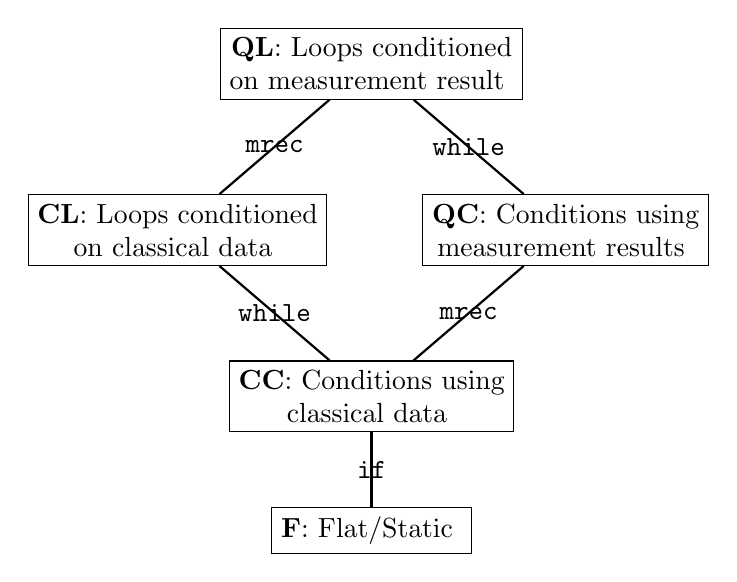
\begin{tikzpicture}
    \node [draw] (ql) at (0,0)                                 [align=center]        {\ccfNode{QL}{Loops conditioned\\ {on measurement result}}};
    \node [draw] [below left  of=ql] [yshift=-40] [xshift=-50] [align=center] (cl)   {\ccfNode{CL}{Loops conditioned\\ {on classical data}}};
    \node [draw] [below right of=ql] [yshift=-40] [xshift=50]  [align=center] (qc)   {\ccfNode{QC}{Conditions using\\ {measurement results}}};
    \node [draw] [below right of=cl] [yshift=-40] [xshift=50]  [align=center] (cc)   {\ccfNode{CC}{Conditions using\\ {classical data}}};
    \node [draw] [below of=cc]       [yshift=-20]                             (flat) {\ccfNode{F}{Flat/Static}};


    \draw [black, thick] (ql) to 
        node[midway] {\texttt{mrec}}
        (cl);

    \draw [black, thick] (ql) to 
        node[midway] {\texttt{while}}
        (qc);
/
    \draw [black, thick] (cc) to 
        node[midway] {\texttt{mrec}}
        (qc);

    \draw [black, thick] (cc) to 
        node[midway] {\texttt{while}}
        (cl);

    \draw [black, thick] (cc) to 
        node[midway] {\texttt{if}}
        (flat);

\end{tikzpicture}
\end{document}                 